\documentclass[a4paper]{book}
\usepackage{makeidx}
\usepackage{graphicx}
\usepackage{multicol}
\usepackage{float}
\usepackage{listings}
\usepackage{color}
\usepackage{textcomp}
\usepackage{alltt}
\usepackage{times}
\usepackage{ifpdf}
\ifpdf
\usepackage[pdftex,
            pagebackref=true,
            colorlinks=true,
            linkcolor=blue,
            unicode
           ]{hyperref}
\else
\usepackage[ps2pdf,
            pagebackref=true,
            colorlinks=true,
            linkcolor=blue,
            unicode
           ]{hyperref}
\usepackage{pspicture}
\fi
\usepackage[utf8]{inputenc}
\usepackage{doxygen}
\lstset{language=C++,inputencoding=utf8,basicstyle=\footnotesize,breaklines=true,breakatwhitespace=true,tabsize=8,numbers=left }
\makeindex
\setcounter{tocdepth}{3}
\renewcommand{\footrulewidth}{0.4pt}
\begin{document}
\hypersetup{pageanchor=false}
\begin{titlepage}
\vspace*{7cm}
\begin{center}
{\Large MessengerSystem \\[1ex]\large 1.0 }\\
\vspace*{1cm}
{\large 作成: Doxygen 1.7.1}\\
\vspace*{0.5cm}
{\small Sun Oct 10 2010 15:18:16}\\
\end{center}
\end{titlepage}
\clearemptydoublepage
\pagenumbering{roman}
\tableofcontents
\clearemptydoublepage
\pagenumbering{arabic}
\hypersetup{pageanchor=true}
\chapter{構成索引}
\section{クラス階層}
この継承一覧はおおまかにはソートされていますが、完全にアルファベット順でソートされてはいません。\begin{DoxyCompactList}
\item \contentsline{section}{MessengerDisplayView}{\pageref{d8/d39/interface_messenger_display_view}}{}
\item \contentsline{section}{MessengerIDGenerator}{\pageref{df/dfd/interface_messenger_i_d_generator}}{}
\item \contentsline{section}{MessengerSystem}{\pageref{dc/dc9/interface_messenger_system}}{}
\begin{DoxyCompactList}
\item \contentsline{section}{MessengerViewController}{\pageref{d7/d34/interface_messenger_view_controller}}{}
\end{DoxyCompactList}
\item \contentsline{section}{MessengerSystemTest}{\pageref{d9/d39/interface_messenger_system_test}}{}
\end{DoxyCompactList}

\chapter{構成索引}
\section{Class List}
Here are the classes, structs, unions and interfaces with brief descriptions:\begin{DoxyCompactList}
\item\contentsline{section}{\hyperlink{structfont_table}{fontTable} }{\pageref{structfont_table}}{}
\item\contentsline{section}{\hyperlink{interface_glyph_table}{GlyphTable} }{\pageref{interface_glyph_table}}{}
\item\contentsline{section}{\hyperlink{interface_messenger_display_view}{MessengerDisplayView} }{\pageref{interface_messenger_display_view}}{}
\item\contentsline{section}{\hyperlink{interface_messenger_i_d_generator}{MessengerIDGenerator} }{\pageref{interface_messenger_i_d_generator}}{}
\item\contentsline{section}{\hyperlink{interface_messenger_system}{MessengerSystem} }{\pageref{interface_messenger_system}}{}
\item\contentsline{section}{\hyperlink{interface_messenger_system_test}{MessengerSystemTest} }{\pageref{interface_messenger_system_test}}{}
\item\contentsline{section}{\hyperlink{interface_messenger_view_controller}{MessengerViewController} }{\pageref{interface_messenger_view_controller}}{}
\end{DoxyCompactList}

\chapter{クラス}
\hypertarget{interface_messenger_display_view}{
\section{MessengerDisplayView Class Reference}
\label{interface_messenger_display_view}\index{MessengerDisplayView@{MessengerDisplayView}}
}


{\ttfamily \#import $<$MessengerDisplayView.h$>$}

\subsection*{Public Member Functions}
\begin{DoxyCompactItemize}
\item 
(void) -\/ \hyperlink{interface_messenger_display_view_ac1aa749dc5f3e7430d8d72841224c919}{setControllerDelegate:}
\item 
(void) -\/ \hyperlink{interface_messenger_display_view_a3790ae1de28d367eb7ec15ec8ed545fb}{updateDrawList:andConnectionList:}
\item 
\hypertarget{interface_messenger_display_view_a35cd00c1a534e3f94111e8ba45bd9cc6}{
(id) -\/ {\bfseries initWithMessengerDisplayFrame:}}
\label{interface_messenger_display_view_a35cd00c1a534e3f94111e8ba45bd9cc6}

\item 
(void) -\/ \hyperlink{interface_messenger_display_view_ad4866b13411e41cdb68d3c92053277eb}{lineFromTo}
\item 
(float) -\/ \hyperlink{interface_messenger_display_view_ac1379b56ac2e7d2b572e147e81971e90}{linePrmGetA}
\item 
\hypertarget{interface_messenger_display_view_a71965f56d6a2665d3f71b0c4ecfe13d0}{
(float) -\/ {\bfseries linePrmGetB}}
\label{interface_messenger_display_view_a71965f56d6a2665d3f71b0c4ecfe13d0}

\item 
\hypertarget{interface_messenger_display_view_ad3b01c0e203aaec5c631091448026ad8}{
(float) -\/ {\bfseries linePrmGetC}}
\label{interface_messenger_display_view_ad3b01c0e203aaec5c631091448026ad8}

\item 
\hypertarget{interface_messenger_display_view_a85472d3e727eb4b6a41ad9f71b83f4f7}{
(CGPoint) -\/ {\bfseries lineCrclCrsPt}}
\label{interface_messenger_display_view_a85472d3e727eb4b6a41ad9f71b83f4f7}

\end{DoxyCompactItemize}
\subsection*{Protected Attributes}
\begin{DoxyCompactItemize}
\item 
\hypertarget{interface_messenger_display_view_aa560737c094fbfbca64d1a52724a307e}{
id {\bfseries m\_\-controllerId}}
\label{interface_messenger_display_view_aa560737c094fbfbca64d1a52724a307e}

\item 
\hypertarget{interface_messenger_display_view_a9329c2b1bc22938abd84560c9a66c89d}{
int {\bfseries m\_\-colorIndex}}
\label{interface_messenger_display_view_a9329c2b1bc22938abd84560c9a66c89d}

\item 
\hypertarget{interface_messenger_display_view_a34409905c6603a9a5084c5248cb3fc2a}{
NSMutableDictionary $\ast$ {\bfseries m\_\-drawList}}
\label{interface_messenger_display_view_a34409905c6603a9a5084c5248cb3fc2a}

\item 
\hypertarget{interface_messenger_display_view_a0b6812fc7734e00008e374c06475511b}{
NSMutableDictionary $\ast$ {\bfseries m\_\-connectionList}}
\label{interface_messenger_display_view_a0b6812fc7734e00008e374c06475511b}

\item 
\hypertarget{interface_messenger_display_view_a1784971ff728fd49f87867555f0d13f9}{
UIEvent $\ast$ {\bfseries m\_\-pinchEvent}}
\label{interface_messenger_display_view_a1784971ff728fd49f87867555f0d13f9}

\item 
\hypertarget{interface_messenger_display_view_a6b0dad3517ee8881c3d4e50c3a130054}{
CGFloat {\bfseries m\_\-lastPinchDist}}
\label{interface_messenger_display_view_a6b0dad3517ee8881c3d4e50c3a130054}

\item 
\hypertarget{interface_messenger_display_view_a13352f8ffc249726f73fcce007df21d0}{
CGPoint {\bfseries m\_\-lastPoint}}
\label{interface_messenger_display_view_a13352f8ffc249726f73fcce007df21d0}

\end{DoxyCompactItemize}


\subsection{Detailed Description}
親となるコントローラから、ボタンをセットされる対象。 ボタンの下敷きに情報、ラインを描く。 

\subsection{Member Function Documentation}
\hypertarget{interface_messenger_display_view_ad4866b13411e41cdb68d3c92053277eb}{
\index{MessengerDisplayView@{MessengerDisplayView}!lineFromTo@{lineFromTo}}
\index{lineFromTo@{lineFromTo}!MessengerDisplayView@{MessengerDisplayView}}
\subsubsection[{lineFromTo}]{\setlength{\rightskip}{0pt plus 5cm}-\/ (void) lineFromTo 
\begin{DoxyParamCaption}
\item[{dummy(CGContextRef)}]{ context}
\item[{(CGPoint)}]{ start}
\item[{(CGPoint)}]{ end}
\item[{(UIColor $\ast$)}]{ color}
\end{DoxyParamCaption}
}}
\label{interface_messenger_display_view_ad4866b13411e41cdb68d3c92053277eb}
ラインを描画するメソッド αは固定。 \hypertarget{interface_messenger_display_view_ac1379b56ac2e7d2b572e147e81971e90}{
\index{MessengerDisplayView@{MessengerDisplayView}!linePrmGetA@{linePrmGetA}}
\index{linePrmGetA@{linePrmGetA}!MessengerDisplayView@{MessengerDisplayView}}
\subsubsection[{linePrmGetA}]{\setlength{\rightskip}{0pt plus 5cm}-\/ (float) linePrmGetA 
\begin{DoxyParamCaption}
\item[{dummy(float)}]{ cx}
\item[{(float)}]{ cy}
\item[{(float)}]{ px}
\item[{(float)}]{ py}
\end{DoxyParamCaption}
}}
\label{interface_messenger_display_view_ac1379b56ac2e7d2b572e147e81971e90}
2点間を通る線について、座標からax+by+c = 0 を出すメソッド \hypertarget{interface_messenger_display_view_ac1aa749dc5f3e7430d8d72841224c919}{
\index{MessengerDisplayView@{MessengerDisplayView}!setControllerDelegate:@{setControllerDelegate:}}
\index{setControllerDelegate:@{setControllerDelegate:}!MessengerDisplayView@{MessengerDisplayView}}
\subsubsection[{setControllerDelegate:}]{\setlength{\rightskip}{0pt plus 5cm}-\/ (void) setControllerDelegate: 
\begin{DoxyParamCaption}
\item[{dummy(id)}]{ contID}
\end{DoxyParamCaption}
}}
\label{interface_messenger_display_view_ac1aa749dc5f3e7430d8d72841224c919}
コントローラのIDをセットする \hypertarget{interface_messenger_display_view_a3790ae1de28d367eb7ec15ec8ed545fb}{
\index{MessengerDisplayView@{MessengerDisplayView}!updateDrawList:andConnectionList:@{updateDrawList:andConnectionList:}}
\index{updateDrawList:andConnectionList:@{updateDrawList:andConnectionList:}!MessengerDisplayView@{MessengerDisplayView}}
\subsubsection[{updateDrawList:andConnectionList:}]{\setlength{\rightskip}{0pt plus 5cm}-\/ (void) updateDrawList: 
\begin{DoxyParamCaption}
\item[{dummy(NSMutableDictionary $\ast$)}]{ draw}
\item[{andConnectionList:(NSMutableDictionary $\ast$)}]{ connect}
\end{DoxyParamCaption}
}}
\label{interface_messenger_display_view_a3790ae1de28d367eb7ec15ec8ed545fb}
辞書を受け取り自己の描画リストを更新する 

The documentation for this class was generated from the following files:\begin{DoxyCompactItemize}
\item 
Classes/MessengerSystem/MessengerDisplayView.h\item 
Classes/MessengerSystem/MessengerDisplayView.m\end{DoxyCompactItemize}

\hypertarget{interface_messenger_i_d_generator}{
\section{クラス MessengerIDGenerator}
\label{df/dfd/interface_messenger_i_d_generator}\index{MessengerIDGenerator@{MessengerIDGenerator}}
}


{\ttfamily \#import $<$MessengerIDGenerator.h$>$}

\subsection*{Static Public メソッド}
\begin{DoxyCompactItemize}
\item 
(NSString $\ast$) + \hyperlink{interface_messenger_i_d_generator_ad0d37385548ddcf8129fde71d41cf8ae}{getMID}
\end{DoxyCompactItemize}


\subsection{説明}
MIDを発行するクラス 特に貯蓄とかはしていない事を明示するために クラスメソッドが一つあるのみ。 

\subsection{関数}
\hypertarget{interface_messenger_i_d_generator_ad0d37385548ddcf8129fde71d41cf8ae}{
\index{MessengerIDGenerator@{MessengerIDGenerator}!getMID@{getMID}}
\index{getMID@{getMID}!MessengerIDGenerator@{MessengerIDGenerator}}
\subsubsection[{getMID}]{\setlength{\rightskip}{0pt plus 5cm}+ (NSString $\ast$) getMID 
\begin{DoxyParamCaption}
{}
\end{DoxyParamCaption}
}}
\label{df/dfd/interface_messenger_i_d_generator_ad0d37385548ddcf8129fde71d41cf8ae}
MID発行メソッド UUIDを作成する 

このクラスの説明は次のファイルから生成されました:\begin{DoxyCompactItemize}
\item 
Classes/MessengerSystem/MessengerIDGenerator.h\item 
Classes/MessengerSystem/MessengerIDGenerator.m\end{DoxyCompactItemize}

\hypertarget{interface_messenger_system}{
\section{クラス MessengerSystem}
\label{dc/dc9/interface_messenger_system}\index{MessengerSystem@{MessengerSystem}}
}
MessengerSystemに対する継承グラフ\begin{figure}[H]
\begin{center}
\leavevmode
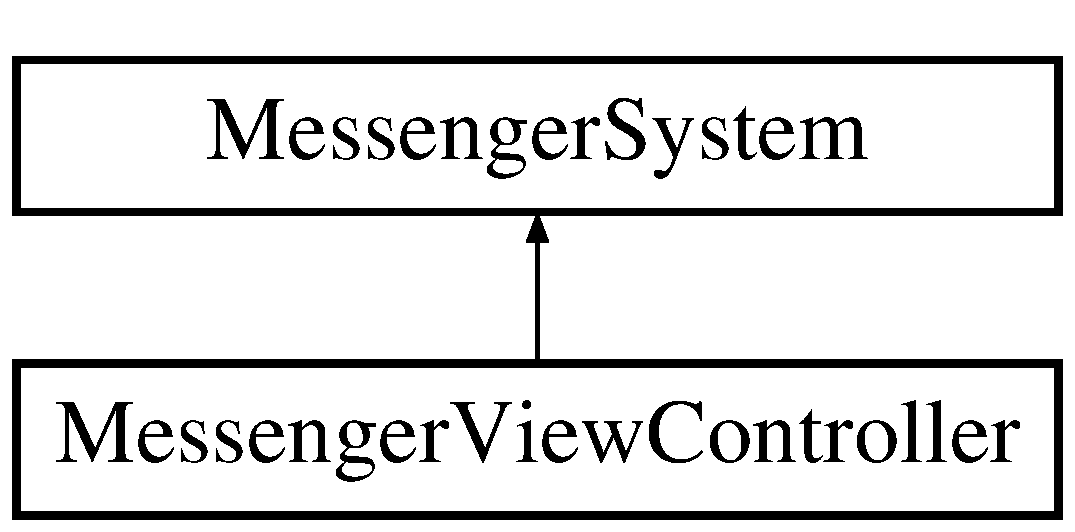
\includegraphics[height=2.000000cm]{dc/dc9/interface_messenger_system}
\end{center}
\end{figure}
\subsection*{Public メソッド}
\begin{DoxyCompactItemize}
\item 
(id) -\/ \hyperlink{interface_messenger_system_a1127377a8d677d41693b435758790e79}{initWithBodyID:withSelector:withName:}
\item 
(id) -\/ \hyperlink{interface_messenger_system_a12fac5bf1d29c2b960e02dab4db80944}{initWithManual}
\item 
(void) -\/ \hyperlink{interface_messenger_system_a2a5f63ed86009e8b451bbbb621e9a94b}{setMyBodyID:}
\item 
(void) -\/ \hyperlink{interface_messenger_system_aafb5a2e5d48a09627f32a4d3c2e3fa29}{setMyBodySelector:}
\item 
(void) -\/ \hyperlink{interface_messenger_system_a2dc1b363d2e1b00f232fd829225a9ff3}{inputParent:}
\item 
(void) -\/ \hyperlink{interface_messenger_system_ae7f62ea0ebdb51b5f2628f3002add7e7}{inputParent:withSpecifiedMID:}
\item 
(void) -\/ \hyperlink{interface_messenger_system_a1b95b2f06c63a72a776c853d74e11b03}{removeFromParent}
\item 
(void) -\/ \hyperlink{interface_messenger_system_abfbdbb7d723b910d012d980daacbcd9b}{removeAllChild}
\item 
(void) -\/ \hyperlink{interface_messenger_system_a0d78a7be460a84be04e67d73ddcf4248}{callMyself:}
\item 
(void) -\/ \hyperlink{interface_messenger_system_ae9f0c6c7daf251eb28aad584b1eca292}{call:withExec:}
\item 
(void) -\/ \hyperlink{interface_messenger_system_ae923fe829663d8974dc34063bd32c4a2}{call:withSpecifiedMID:withExec:}
\item 
(void) -\/ \hyperlink{interface_messenger_system_acf758deab41281c54d928be2a72fc9ba}{callParent:}
\item 
(NSDictionary $\ast$) -\/ \hyperlink{interface_messenger_system_ad4e20b8da148b72f520986386c7fb8a5}{tag:val:}
\item 
(NSDictionary $\ast$) -\/ \hyperlink{interface_messenger_system_ad7b796c0354f4a6f380392421d4abc0d}{withRemoteFrom:withSelector:}
\item 
(NSDictionary $\ast$) -\/ \hyperlink{interface_messenger_system_ac424d46f571c01154893e4747a665930}{withDelay:}
\item 
(void) -\/ \hyperlink{interface_messenger_system_aaaa066451fb04c37c88e6a7efc94c63e}{remoteInvocation:}
\item 
(NSMutableDictionary $\ast$) -\/ \hyperlink{interface_messenger_system_a857e1c7932fdb366b52b687832c8e0bf}{getLogStore}
\item 
(NSMutableDictionary $\ast$) -\/ \hyperlink{interface_messenger_system_a057d907e4e7325c927580ace6701f95c}{getChildDict}
\item 
(NSString $\ast$) -\/ \hyperlink{interface_messenger_system_a1a0013cb76d7f354e7d71e09e0456766}{getExecAsString:}
\item 
(int) -\/ \hyperlink{interface_messenger_system_aef3cf1f4d71c77f66e6053dcd277beba}{getExecAsIntFromDict:}
\item 
(int) -\/ \hyperlink{interface_messenger_system_a881655597ee31052ca7cd72acd1343c2}{getIntFromExec:}
\item 
(int) -\/ \hyperlink{interface_messenger_system_a9c32da2a99a87a32c2567b29b4d411ac}{changeStrToNumber:}
\item 
(NSString $\ast$) -\/ \hyperlink{interface_messenger_system_ace36dcb764d249819d4ea85fac0afe5c}{changeNumberToStr:}
\item 
(BOOL) -\/ \hyperlink{interface_messenger_system_a4ab801cff2356929a18a551b3537f435}{hasParent}
\item 
(BOOL) -\/ \hyperlink{interface_messenger_system_a9db1bcbbaf0abb9e8e1af5a2aa5bf9fa}{hasChild}
\item 
(BOOL) -\/ \hyperlink{interface_messenger_system_a975357de1acaa17f15d90e67d0203ff4}{isIncludeRemote:}
\item 
(id) -\/ \hyperlink{interface_messenger_system_a7ebd928ddb4092333370af98d34095ed}{getMyBodyID}
\item 
(SEL) -\/ \hyperlink{interface_messenger_system_a0c021c0bc0628174e8b16f664205ebf6}{getMyBodySelector}
\item 
(NSString $\ast$) -\/ \hyperlink{interface_messenger_system_a8d6c34458dcb7c44337b68b2c47c9050}{getMyName}
\item 
(NSString $\ast$) -\/ \hyperlink{interface_messenger_system_a53fb306c1c478aafd66a039cf08e9f53}{getMyMID}
\item 
(NSString $\ast$) -\/ \hyperlink{interface_messenger_system_a8480affbc74b87d15b301d5b32681a70}{getMyParentName}
\item 
(NSString $\ast$) -\/ \hyperlink{interface_messenger_system_a59c153b480be68325af6a66f18cecd0b}{getMyParentMID}
\item 
(void) -\/ \hyperlink{interface_messenger_system_a6ffde31c3597bd083b47e30d26eb926f}{cancelPerform}
\item 
(BOOL) -\/ \hyperlink{interface_messenger_system_adcebdb1f9788a0bb75bb4c0433849ace}{isReleasable}
\item 
\hypertarget{interface_messenger_system_acd15a25f39e26b450bb1c33edd1f2d51}{
(void) -\/ {\bfseries innerPerform:}}
\label{dc/dc9/interface_messenger_system_acd15a25f39e26b450bb1c33edd1f2d51}

\item 
\hypertarget{interface_messenger_system_a60cbd00cd24aa502aa77d86e4391a1b7}{
(void) -\/ {\bfseries sendPerform:}}
\label{dc/dc9/interface_messenger_system_a60cbd00cd24aa502aa77d86e4391a1b7}

\item 
\hypertarget{interface_messenger_system_a12e9a8d84b6cb12f55bf7453166cfab1}{
(void) -\/ {\bfseries sendPerform:withDelay:}}
\label{dc/dc9/interface_messenger_system_a12e9a8d84b6cb12f55bf7453166cfab1}

\item 
\hypertarget{interface_messenger_system_a0938a6c892b3a634870238b4555dc921}{
(void) -\/ {\bfseries sendMessage:}}
\label{dc/dc9/interface_messenger_system_a0938a6c892b3a634870238b4555dc921}

\item 
\hypertarget{interface_messenger_system_a51502df160822ba7c6fd754fdc6353de}{
(void) -\/ {\bfseries remoteInvocation:withDict:}}
\label{dc/dc9/interface_messenger_system_a51502df160822ba7c6fd754fdc6353de}

\item 
\hypertarget{interface_messenger_system_a7e77f9abb100c6123caaa291d7f92ffb}{
(void) -\/ {\bfseries createdNotice}}
\label{dc/dc9/interface_messenger_system_a7e77f9abb100c6123caaa291d7f92ffb}

\item 
\hypertarget{interface_messenger_system_a28703ac96f244da4d7c62207cf65ff69}{
(void) -\/ {\bfseries updatedNotice:withParentMID:}}
\label{dc/dc9/interface_messenger_system_a28703ac96f244da4d7c62207cf65ff69}

\item 
\hypertarget{interface_messenger_system_a127cce35cc1c079fed1bceecccf23a66}{
(void) -\/ {\bfseries killedNotice}}
\label{dc/dc9/interface_messenger_system_a127cce35cc1c079fed1bceecccf23a66}

\item 
\hypertarget{interface_messenger_system_a57dd4208efc5d477c50c5c5f55fe7ff1}{
(void) -\/ {\bfseries setChildDictChildNameAsValue:withMIDAsKey:}}
\label{dc/dc9/interface_messenger_system_a57dd4208efc5d477c50c5c5f55fe7ff1}

\item 
\hypertarget{interface_messenger_system_aadeb829f6e394bbc36d77593ed6fe677}{
(void) -\/ {\bfseries removeChildDictChildNameAsValue:withMIDAsKey:}}
\label{dc/dc9/interface_messenger_system_aadeb829f6e394bbc36d77593ed6fe677}

\item 
\hypertarget{interface_messenger_system_a4ea61787df15874f8db773d159b6d10c}{
(NSDictionary $\ast$) -\/ {\bfseries setPrivateRemoteInvocationFrom:withSelector:}}
\label{dc/dc9/interface_messenger_system_a4ea61787df15874f8db773d159b6d10c}

\item 
\hypertarget{interface_messenger_system_a60c9a5dc9cf6d420d944edead0c957d8}{
(NSDictionary $\ast$) -\/ {\bfseries setRemoteInvocationFrom:withSelector:}}
\label{dc/dc9/interface_messenger_system_a60c9a5dc9cf6d420d944edead0c957d8}

\item 
\hypertarget{interface_messenger_system_aa4f4f9dbed2ccb22b30fa3bc86229560}{
(void) -\/ {\bfseries addCreationLog:}}
\label{dc/dc9/interface_messenger_system_aa4f4f9dbed2ccb22b30fa3bc86229560}

\item 
\hypertarget{interface_messenger_system_aea64a6b2e2486edb5a3443a23d13934f}{
(void) -\/ {\bfseries saveLogForReceived:}}
\label{dc/dc9/interface_messenger_system_aea64a6b2e2486edb5a3443a23d13934f}

\item 
\hypertarget{interface_messenger_system_a51d6be48e11ee01ba98c720b46ae398e}{
(NSMutableDictionary $\ast$) -\/ {\bfseries createLogForReply}}
\label{dc/dc9/interface_messenger_system_a51d6be48e11ee01ba98c720b46ae398e}

\item 
\hypertarget{interface_messenger_system_a04b3995de0fb3486ee1f64bc8868b8f3}{
(void) -\/ {\bfseries saveToLogStore:log:}}
\label{dc/dc9/interface_messenger_system_a04b3995de0fb3486ee1f64bc8868b8f3}

\item 
\hypertarget{interface_messenger_system_a0388f0bc3b5d73f8404fb65ae9f2478d}{
(void) -\/ {\bfseries setMyName:}}
\label{dc/dc9/interface_messenger_system_a0388f0bc3b5d73f8404fb65ae9f2478d}

\item 
\hypertarget{interface_messenger_system_adac10123acd489108d70a63d1b42669c}{
(void) -\/ {\bfseries initMyMID}}
\label{dc/dc9/interface_messenger_system_adac10123acd489108d70a63d1b42669c}

\item 
\hypertarget{interface_messenger_system_ae32a19a0477498f6b079551dfa08a15e}{
(void) -\/ {\bfseries initMyParentData}}
\label{dc/dc9/interface_messenger_system_ae32a19a0477498f6b079551dfa08a15e}

\item 
\hypertarget{interface_messenger_system_a111b446c0453facea8fc35774323dae7}{
(void) -\/ {\bfseries resetMyParentData}}
\label{dc/dc9/interface_messenger_system_a111b446c0453facea8fc35774323dae7}

\item 
\hypertarget{interface_messenger_system_a77cb388881cfe26e1b6440a1409c7c23}{
(void) -\/ {\bfseries setMyParentName:}}
\label{dc/dc9/interface_messenger_system_a77cb388881cfe26e1b6440a1409c7c23}

\item 
\hypertarget{interface_messenger_system_a4b835de059160b6e22eadd4035769c04}{
(void) -\/ {\bfseries setMyParentMID:}}
\label{dc/dc9/interface_messenger_system_a4b835de059160b6e22eadd4035769c04}

\end{DoxyCompactItemize}
\subsection*{Static Public メソッド}
\begin{DoxyCompactItemize}
\item 
(NSString $\ast$) + \hyperlink{interface_messenger_system_aebad51a1ea3a010f1bb20d2f3327adcc}{version}
\end{DoxyCompactItemize}
\subsection*{Protected 変数}
\begin{DoxyCompactItemize}
\item 
\hypertarget{interface_messenger_system_a90f9745297d9d34f403579d395744a71}{
id {\bfseries myBodyID}}
\label{dc/dc9/interface_messenger_system_a90f9745297d9d34f403579d395744a71}

\item 
\hypertarget{interface_messenger_system_a469a5e545f12673594bc0117c8441068}{
SEL {\bfseries myBodySelector}}
\label{dc/dc9/interface_messenger_system_a469a5e545f12673594bc0117c8441068}

\item 
\hypertarget{interface_messenger_system_aa6f745c063b7432f33409c4e74fad099}{
NSString $\ast$ {\bfseries myName}}
\label{dc/dc9/interface_messenger_system_aa6f745c063b7432f33409c4e74fad099}

\item 
\hypertarget{interface_messenger_system_ab0873dccec01721962a9feda60f881e9}{
NSString $\ast$ {\bfseries myMID}}
\label{dc/dc9/interface_messenger_system_ab0873dccec01721962a9feda60f881e9}

\item 
\hypertarget{interface_messenger_system_a768d13ac0ab2689e095bcae527cb3c1b}{
NSString $\ast$ {\bfseries myParentName}}
\label{dc/dc9/interface_messenger_system_a768d13ac0ab2689e095bcae527cb3c1b}

\item 
\hypertarget{interface_messenger_system_a160a088edbe00c0a701b5c51a36203d3}{
NSString $\ast$ {\bfseries myParentMID}}
\label{dc/dc9/interface_messenger_system_a160a088edbe00c0a701b5c51a36203d3}

\item 
\hypertarget{interface_messenger_system_a7596fd096f620d0141fac502665dcabf}{
NSMutableDictionary $\ast$ {\bfseries m\_\-childDict}}
\label{dc/dc9/interface_messenger_system_a7596fd096f620d0141fac502665dcabf}

\item 
\hypertarget{interface_messenger_system_adf17d60a0ff5e2c21cb2f3717d9b5b55}{
NSMutableDictionary $\ast$ {\bfseries m\_\-logDict}}
\label{dc/dc9/interface_messenger_system_adf17d60a0ff5e2c21cb2f3717d9b5b55}

\end{DoxyCompactItemize}


\subsection{説明}
プライベート実装

パブリック実装 

\subsection{関数}
\hypertarget{interface_messenger_system_ae9f0c6c7daf251eb28aad584b1eca292}{
\index{MessengerSystem@{MessengerSystem}!call:withExec:@{call:withExec:}}
\index{call:withExec:@{call:withExec:}!MessengerSystem@{MessengerSystem}}
\subsubsection[{call:withExec:}]{\setlength{\rightskip}{0pt plus 5cm}-\/ (void) call: 
\begin{DoxyParamCaption}
\item[{dummy(NSString $\ast$)}]{ childName}
\item[{withExec:(NSString $\ast$)}]{ exec}
\item[{,}]{ ...}
\end{DoxyParamCaption}
}}
\label{dc/dc9/interface_messenger_system_ae9f0c6c7daf251eb28aad584b1eca292}
特定の名前のmessengerへの通信を行うメソッド 異なる名前の親から子へのメッセージ限定 

\hyperlink{interface_messenger_view_controller_a7a416a5ec2bcd17f259e1b2fc017d6a6}{MessengerViewController}で再定義されています。

\hypertarget{interface_messenger_system_ae923fe829663d8974dc34063bd32c4a2}{
\index{MessengerSystem@{MessengerSystem}!call:withSpecifiedMID:withExec:@{call:withSpecifiedMID:withExec:}}
\index{call:withSpecifiedMID:withExec:@{call:withSpecifiedMID:withExec:}!MessengerSystem@{MessengerSystem}}
\subsubsection[{call:withSpecifiedMID:withExec:}]{\setlength{\rightskip}{0pt plus 5cm}-\/ (void) call: 
\begin{DoxyParamCaption}
\item[{dummy(NSString $\ast$)}]{ childName}
\item[{withSpecifiedMID:(NSString $\ast$)}]{ mID}
\item[{withExec:(NSString $\ast$)}]{ exec}
\item[{,}]{ ...}
\end{DoxyParamCaption}
}}
\label{dc/dc9/interface_messenger_system_ae923fe829663d8974dc34063bd32c4a2}
特定の子への通信を行うメソッド、特にMIDを使い、相手を最大限特定する。 \hypertarget{interface_messenger_system_a0d78a7be460a84be04e67d73ddcf4248}{
\index{MessengerSystem@{MessengerSystem}!callMyself:@{callMyself:}}
\index{callMyself:@{callMyself:}!MessengerSystem@{MessengerSystem}}
\subsubsection[{callMyself:}]{\setlength{\rightskip}{0pt plus 5cm}-\/ (void) callMyself: 
\begin{DoxyParamCaption}
\item[{dummy(NSString $\ast$)}]{ exec}
\item[{,}]{ ...}
\end{DoxyParamCaption}
}}
\label{dc/dc9/interface_messenger_system_a0d78a7be460a84be04e67d73ddcf4248}
自分自身のmessengerへと通信を行うメソッド 

\hyperlink{interface_messenger_view_controller_a416d9acd2e8346b9ab8870b64571f322}{MessengerViewController}で再定義されています。

\hypertarget{interface_messenger_system_acf758deab41281c54d928be2a72fc9ba}{
\index{MessengerSystem@{MessengerSystem}!callParent:@{callParent:}}
\index{callParent:@{callParent:}!MessengerSystem@{MessengerSystem}}
\subsubsection[{callParent:}]{\setlength{\rightskip}{0pt plus 5cm}-\/ (void) callParent: 
\begin{DoxyParamCaption}
\item[{dummy(NSString $\ast$)}]{ exec}
\item[{,}]{ ...}
\end{DoxyParamCaption}
}}
\label{dc/dc9/interface_messenger_system_acf758deab41281c54d928be2a72fc9ba}
親への通信を行うメソッド 

\hyperlink{interface_messenger_view_controller_afa8cf33ccddb2f83e214b192707bdbd6}{MessengerViewController}で再定義されています。

\hypertarget{interface_messenger_system_a6ffde31c3597bd083b47e30d26eb926f}{
\index{MessengerSystem@{MessengerSystem}!cancelPerform@{cancelPerform}}
\index{cancelPerform@{cancelPerform}!MessengerSystem@{MessengerSystem}}
\subsubsection[{cancelPerform}]{\setlength{\rightskip}{0pt plus 5cm}-\/ (void) cancelPerform 
\begin{DoxyParamCaption}
{}
\end{DoxyParamCaption}
}}
\label{dc/dc9/interface_messenger_system_a6ffde31c3597bd083b47e30d26eb926f}
遅延実行をキャンセルするメソッド \hypertarget{interface_messenger_system_ace36dcb764d249819d4ea85fac0afe5c}{
\index{MessengerSystem@{MessengerSystem}!changeNumberToStr:@{changeNumberToStr:}}
\index{changeNumberToStr:@{changeNumberToStr:}!MessengerSystem@{MessengerSystem}}
\subsubsection[{changeNumberToStr:}]{\setlength{\rightskip}{0pt plus 5cm}-\/ (NSString $\ast$) changeNumberToStr: 
\begin{DoxyParamCaption}
\item[{dummy(int)}]{ num}
\end{DoxyParamCaption}
}}
\label{dc/dc9/interface_messenger_system_ace36dcb764d249819d4ea85fac0afe5c}
数値の文字列化

数値の文字列化 出来ません。ロジック的に不可逆。 

数字の4文字をまとめて処理している。最小で1,とかなので、足したものから複合するしかない。或る意味暗号。

\hypertarget{interface_messenger_system_a9c32da2a99a87a32c2567b29b4d411ac}{
\index{MessengerSystem@{MessengerSystem}!changeStrToNumber:@{changeStrToNumber:}}
\index{changeStrToNumber:@{changeStrToNumber:}!MessengerSystem@{MessengerSystem}}
\subsubsection[{changeStrToNumber:}]{\setlength{\rightskip}{0pt plus 5cm}-\/ (int) changeStrToNumber: 
\begin{DoxyParamCaption}
\item[{dummy(NSString $\ast$)}]{ str}
\end{DoxyParamCaption}
}}
\label{dc/dc9/interface_messenger_system_a9c32da2a99a87a32c2567b29b4d411ac}
ストリングの数値化

文字列の数値化 \hypertarget{interface_messenger_system_a057d907e4e7325c927580ace6701f95c}{
\index{MessengerSystem@{MessengerSystem}!getChildDict@{getChildDict}}
\index{getChildDict@{getChildDict}!MessengerSystem@{MessengerSystem}}
\subsubsection[{getChildDict}]{\setlength{\rightskip}{0pt plus 5cm}-\/ (NSMutableDictionary $\ast$) getChildDict 
\begin{DoxyParamCaption}
{}
\end{DoxyParamCaption}
}}
\label{dc/dc9/interface_messenger_system_a057d907e4e7325c927580ace6701f95c}
子供辞書の取得

m\_\-childDictを返す \hypertarget{interface_messenger_system_aef3cf1f4d71c77f66e6053dcd277beba}{
\index{MessengerSystem@{MessengerSystem}!getExecAsIntFromDict:@{getExecAsIntFromDict:}}
\index{getExecAsIntFromDict:@{getExecAsIntFromDict:}!MessengerSystem@{MessengerSystem}}
\subsubsection[{getExecAsIntFromDict:}]{\setlength{\rightskip}{0pt plus 5cm}-\/ (int) getExecAsIntFromDict: 
\begin{DoxyParamCaption}
\item[{dummy(NSMutableDictionary $\ast$)}]{ dict}
\end{DoxyParamCaption}
}}
\label{dc/dc9/interface_messenger_system_aef3cf1f4d71c77f66e6053dcd277beba}
コマンド情報を数値で取得する 辞書からswitch文で使用する数値を取得する

実行処理名を指定、Int値を取得する この時点で飛び込んでくるストリングのポインタと同じ値を直前で出して、合致する値を出せればいいのか、、って定数じゃないが、、一致は出来る、、うーん。 \hypertarget{interface_messenger_system_a1a0013cb76d7f354e7d71e09e0456766}{
\index{MessengerSystem@{MessengerSystem}!getExecAsString:@{getExecAsString:}}
\index{getExecAsString:@{getExecAsString:}!MessengerSystem@{MessengerSystem}}
\subsubsection[{getExecAsString:}]{\setlength{\rightskip}{0pt plus 5cm}-\/ (NSString $\ast$) getExecAsString: 
\begin{DoxyParamCaption}
\item[{dummy(NSMutableDictionary $\ast$)}]{ dict}
\end{DoxyParamCaption}
}}
\label{dc/dc9/interface_messenger_system_a1a0013cb76d7f354e7d71e09e0456766}
コマンド情報を文字列で取得する

実行処理名を指定、String値を取得する \hypertarget{interface_messenger_system_a881655597ee31052ca7cd72acd1343c2}{
\index{MessengerSystem@{MessengerSystem}!getIntFromExec:@{getIntFromExec:}}
\index{getIntFromExec:@{getIntFromExec:}!MessengerSystem@{MessengerSystem}}
\subsubsection[{getIntFromExec:}]{\setlength{\rightskip}{0pt plus 5cm}-\/ (int) getIntFromExec: 
\begin{DoxyParamCaption}
\item[{dummy(NSString $\ast$)}]{ exec}
\end{DoxyParamCaption}
}}
\label{dc/dc9/interface_messenger_system_a881655597ee31052ca7cd72acd1343c2}
文字列からswitch文で使用する数値を取得する

NSStringからInt値を出す \hypertarget{interface_messenger_system_a857e1c7932fdb366b52b687832c8e0bf}{
\index{MessengerSystem@{MessengerSystem}!getLogStore@{getLogStore}}
\index{getLogStore@{getLogStore}!MessengerSystem@{MessengerSystem}}
\subsubsection[{getLogStore}]{\setlength{\rightskip}{0pt plus 5cm}-\/ (NSMutableDictionary $\ast$) getLogStore 
\begin{DoxyParamCaption}
{}
\end{DoxyParamCaption}
}}
\label{dc/dc9/interface_messenger_system_a857e1c7932fdb366b52b687832c8e0bf}
ログストアの取得

観察用にこのmessengerに書かれているログを取得するメソッド \hypertarget{interface_messenger_system_a7ebd928ddb4092333370af98d34095ed}{
\index{MessengerSystem@{MessengerSystem}!getMyBodyID@{getMyBodyID}}
\index{getMyBodyID@{getMyBodyID}!MessengerSystem@{MessengerSystem}}
\subsubsection[{getMyBodyID}]{\setlength{\rightskip}{0pt plus 5cm}-\/ (id) getMyBodyID 
\begin{DoxyParamCaption}
{}
\end{DoxyParamCaption}
}}
\label{dc/dc9/interface_messenger_system_a7ebd928ddb4092333370af98d34095ed}
クラスが持つ値の ゲッター

自分のBodyIDを返すメソッド \hypertarget{interface_messenger_system_a0c021c0bc0628174e8b16f664205ebf6}{
\index{MessengerSystem@{MessengerSystem}!getMyBodySelector@{getMyBodySelector}}
\index{getMyBodySelector@{getMyBodySelector}!MessengerSystem@{MessengerSystem}}
\subsubsection[{getMyBodySelector}]{\setlength{\rightskip}{0pt plus 5cm}-\/ (SEL) getMyBodySelector 
\begin{DoxyParamCaption}
{}
\end{DoxyParamCaption}
}}
\label{dc/dc9/interface_messenger_system_a0c021c0bc0628174e8b16f664205ebf6}
自分のセレクター用ポインタを返すメソッド \hypertarget{interface_messenger_system_a53fb306c1c478aafd66a039cf08e9f53}{
\index{MessengerSystem@{MessengerSystem}!getMyMID@{getMyMID}}
\index{getMyMID@{getMyMID}!MessengerSystem@{MessengerSystem}}
\subsubsection[{getMyMID}]{\setlength{\rightskip}{0pt plus 5cm}-\/ (NSString $\ast$) getMyMID 
\begin{DoxyParamCaption}
{}
\end{DoxyParamCaption}
}}
\label{dc/dc9/interface_messenger_system_a53fb306c1c478aafd66a039cf08e9f53}
自分のMIDを返すメソッド \hypertarget{interface_messenger_system_a8d6c34458dcb7c44337b68b2c47c9050}{
\index{MessengerSystem@{MessengerSystem}!getMyName@{getMyName}}
\index{getMyName@{getMyName}!MessengerSystem@{MessengerSystem}}
\subsubsection[{getMyName}]{\setlength{\rightskip}{0pt plus 5cm}-\/ (NSString $\ast$) getMyName 
\begin{DoxyParamCaption}
{}
\end{DoxyParamCaption}
}}
\label{dc/dc9/interface_messenger_system_a8d6c34458dcb7c44337b68b2c47c9050}
自分の名称を返すメソッド \hypertarget{interface_messenger_system_a59c153b480be68325af6a66f18cecd0b}{
\index{MessengerSystem@{MessengerSystem}!getMyParentMID@{getMyParentMID}}
\index{getMyParentMID@{getMyParentMID}!MessengerSystem@{MessengerSystem}}
\subsubsection[{getMyParentMID}]{\setlength{\rightskip}{0pt plus 5cm}-\/ (NSString $\ast$) getMyParentMID 
\begin{DoxyParamCaption}
{}
\end{DoxyParamCaption}
}}
\label{dc/dc9/interface_messenger_system_a59c153b480be68325af6a66f18cecd0b}
親のMIDを返すメソッド \hypertarget{interface_messenger_system_a8480affbc74b87d15b301d5b32681a70}{
\index{MessengerSystem@{MessengerSystem}!getMyParentName@{getMyParentName}}
\index{getMyParentName@{getMyParentName}!MessengerSystem@{MessengerSystem}}
\subsubsection[{getMyParentName}]{\setlength{\rightskip}{0pt plus 5cm}-\/ (NSString $\ast$) getMyParentName 
\begin{DoxyParamCaption}
{}
\end{DoxyParamCaption}
}}
\label{dc/dc9/interface_messenger_system_a8480affbc74b87d15b301d5b32681a70}
親の名称を返すメソッド \hypertarget{interface_messenger_system_a9db1bcbbaf0abb9e8e1af5a2aa5bf9fa}{
\index{MessengerSystem@{MessengerSystem}!hasChild@{hasChild}}
\index{hasChild@{hasChild}!MessengerSystem@{MessengerSystem}}
\subsubsection[{hasChild}]{\setlength{\rightskip}{0pt plus 5cm}-\/ (BOOL) hasChild 
\begin{DoxyParamCaption}
{}
\end{DoxyParamCaption}
}}
\label{dc/dc9/interface_messenger_system_a9db1bcbbaf0abb9e8e1af5a2aa5bf9fa}
子供が設定されているか否か返す \hypertarget{interface_messenger_system_a4ab801cff2356929a18a551b3537f435}{
\index{MessengerSystem@{MessengerSystem}!hasParent@{hasParent}}
\index{hasParent@{hasParent}!MessengerSystem@{MessengerSystem}}
\subsubsection[{hasParent}]{\setlength{\rightskip}{0pt plus 5cm}-\/ (BOOL) hasParent 
\begin{DoxyParamCaption}
{}
\end{DoxyParamCaption}
}}
\label{dc/dc9/interface_messenger_system_a4ab801cff2356929a18a551b3537f435}
ユーティリティ

親が設定されているか否か返す \hypertarget{interface_messenger_system_a1127377a8d677d41693b435758790e79}{
\index{MessengerSystem@{MessengerSystem}!initWithBodyID:withSelector:withName:@{initWithBodyID:withSelector:withName:}}
\index{initWithBodyID:withSelector:withName:@{initWithBodyID:withSelector:withName:}!MessengerSystem@{MessengerSystem}}
\subsubsection[{initWithBodyID:withSelector:withName:}]{\setlength{\rightskip}{0pt plus 5cm}-\/ (id) initWithBodyID: 
\begin{DoxyParamCaption}
\item[{dummy(id)}]{ body\_\-id}
\item[{withSelector:(SEL)}]{ body\_\-selector}
\item[{withName:(NSString $\ast$)}]{ name}
\end{DoxyParamCaption}
}}
\label{dc/dc9/interface_messenger_system_a1127377a8d677d41693b435758790e79}
MessengerSystemインスタンスの初期化メソッド

body\_\-id:このインスタンスを所持するオブジェクトのID body\_\-selector:このインスタンスを所持するオブジェクトが自動的に呼び出してほしいメソッドのselector name:このメッセンジャーの名称 

\hyperlink{interface_messenger_view_controller_a44c0a2552e50d6223a8230447be3e83a}{MessengerViewController}で再定義されています。

\hypertarget{interface_messenger_system_a12fac5bf1d29c2b960e02dab4db80944}{
\index{MessengerSystem@{MessengerSystem}!initWithManual@{initWithManual}}
\index{initWithManual@{initWithManual}!MessengerSystem@{MessengerSystem}}
\subsubsection[{initWithManual}]{\setlength{\rightskip}{0pt plus 5cm}-\/ (id) initWithManual 
\begin{DoxyParamCaption}
{}
\end{DoxyParamCaption}
}}
\label{dc/dc9/interface_messenger_system_a12fac5bf1d29c2b960e02dab4db80944}
マニュアルを初期化、表示するプログラム 文字のみ。 \hypertarget{interface_messenger_system_a2dc1b363d2e1b00f232fd829225a9ff3}{
\index{MessengerSystem@{MessengerSystem}!inputParent:@{inputParent:}}
\index{inputParent:@{inputParent:}!MessengerSystem@{MessengerSystem}}
\subsubsection[{inputParent:}]{\setlength{\rightskip}{0pt plus 5cm}-\/ (void) inputParent: 
\begin{DoxyParamCaption}
\item[{dummy(NSString $\ast$)}]{ parentName}
\end{DoxyParamCaption}
}}
\label{dc/dc9/interface_messenger_system_a2dc1b363d2e1b00f232fd829225a9ff3}
親へと自分が子供である事の通知を行い、返り値として親のMIDをmyParentMIDとして受け取るメソッド 受け取り用のメソッドの情報を親へと渡し、親からの遠隔MID入力を受ける。 

\hyperlink{interface_messenger_view_controller_a33bb3cca76fba84a3e5b480131e5faf1}{MessengerViewController}で再定義されています。

\hypertarget{interface_messenger_system_ae7f62ea0ebdb51b5f2628f3002add7e7}{
\index{MessengerSystem@{MessengerSystem}!inputParent:withSpecifiedMID:@{inputParent:withSpecifiedMID:}}
\index{inputParent:withSpecifiedMID:@{inputParent:withSpecifiedMID:}!MessengerSystem@{MessengerSystem}}
\subsubsection[{inputParent:withSpecifiedMID:}]{\setlength{\rightskip}{0pt plus 5cm}-\/ (void) inputParent: 
\begin{DoxyParamCaption}
\item[{dummy(NSString $\ast$)}]{ parent}
\item[{withSpecifiedMID:(NSString $\ast$)}]{ mID}
\end{DoxyParamCaption}
}}
\label{dc/dc9/interface_messenger_system_ae7f62ea0ebdb51b5f2628f3002add7e7}
親へと自分が子供である事の通知を行い、返り値として親のMIDをmyParentMIDとして受け取るメソッド 親のMIDを特に特定できる場合に使用する。 \hypertarget{interface_messenger_system_a975357de1acaa17f15d90e67d0203ff4}{
\index{MessengerSystem@{MessengerSystem}!isIncludeRemote:@{isIncludeRemote:}}
\index{isIncludeRemote:@{isIncludeRemote:}!MessengerSystem@{MessengerSystem}}
\subsubsection[{isIncludeRemote:}]{\setlength{\rightskip}{0pt plus 5cm}-\/ (BOOL) isIncludeRemote: 
\begin{DoxyParamCaption}
\item[{dummy(NSMutableDictionary $\ast$)}]{ dict}
\end{DoxyParamCaption}
}}
\label{dc/dc9/interface_messenger_system_a975357de1acaa17f15d90e67d0203ff4}
遠隔実行のコマンドがメッセージに含まれているか

受け取ったデータに遠隔実行が含まれているか否か返す \hypertarget{interface_messenger_system_adcebdb1f9788a0bb75bb4c0433849ace}{
\index{MessengerSystem@{MessengerSystem}!isReleasable@{isReleasable}}
\index{isReleasable@{isReleasable}!MessengerSystem@{MessengerSystem}}
\subsubsection[{isReleasable}]{\setlength{\rightskip}{0pt plus 5cm}-\/ (BOOL) isReleasable 
\begin{DoxyParamCaption}
{}
\end{DoxyParamCaption}
}}
\label{dc/dc9/interface_messenger_system_adcebdb1f9788a0bb75bb4c0433849ace}
メッセンジャーが解放可能かどうか、取得するメソッド \hypertarget{interface_messenger_system_aaaa066451fb04c37c88e6a7efc94c63e}{
\index{MessengerSystem@{MessengerSystem}!remoteInvocation:@{remoteInvocation:}}
\index{remoteInvocation:@{remoteInvocation:}!MessengerSystem@{MessengerSystem}}
\subsubsection[{remoteInvocation:}]{\setlength{\rightskip}{0pt plus 5cm}-\/ (void) remoteInvocation: 
\begin{DoxyParamCaption}
\item[{dummy(NSMutableDictionary $\ast$)}]{ dict}
\item[{,}]{ ...}
\end{DoxyParamCaption}
}}
\label{dc/dc9/interface_messenger_system_aaaa066451fb04c37c88e6a7efc94c63e}
遠隔実行実装

遠隔実行実装 パブリック用 \hypertarget{interface_messenger_system_abfbdbb7d723b910d012d980daacbcd9b}{
\index{MessengerSystem@{MessengerSystem}!removeAllChild@{removeAllChild}}
\index{removeAllChild@{removeAllChild}!MessengerSystem@{MessengerSystem}}
\subsubsection[{removeAllChild}]{\setlength{\rightskip}{0pt plus 5cm}-\/ (void) removeAllChild 
\begin{DoxyParamCaption}
{}
\end{DoxyParamCaption}
}}
\label{dc/dc9/interface_messenger_system_abfbdbb7d723b910d012d980daacbcd9b}
子供との関連性を解除する 自分の事を親に設定している全てのオブジェクトから離脱するブロードコールを行う。 \hypertarget{interface_messenger_system_a1b95b2f06c63a72a776c853d74e11b03}{
\index{MessengerSystem@{MessengerSystem}!removeFromParent@{removeFromParent}}
\index{removeFromParent@{removeFromParent}!MessengerSystem@{MessengerSystem}}
\subsubsection[{removeFromParent}]{\setlength{\rightskip}{0pt plus 5cm}-\/ (void) removeFromParent 
\begin{DoxyParamCaption}
{}
\end{DoxyParamCaption}
}}
\label{dc/dc9/interface_messenger_system_a1b95b2f06c63a72a776c853d74e11b03}
現在の親情報を削除する \hypertarget{interface_messenger_system_a2a5f63ed86009e8b451bbbb621e9a94b}{
\index{MessengerSystem@{MessengerSystem}!setMyBodyID:@{setMyBodyID:}}
\index{setMyBodyID:@{setMyBodyID:}!MessengerSystem@{MessengerSystem}}
\subsubsection[{setMyBodyID:}]{\setlength{\rightskip}{0pt plus 5cm}-\/ (void) setMyBodyID: 
\begin{DoxyParamCaption}
\item[{dummy(id)}]{ bodyID}
\end{DoxyParamCaption}
}}
\label{dc/dc9/interface_messenger_system_a2a5f63ed86009e8b451bbbb621e9a94b}
自分のBodyIDをセットするメソッド 

\hyperlink{interface_messenger_view_controller_abab9347cc7ed46bd04978ca00e081a0e}{MessengerViewController}で再定義されています。

\hypertarget{interface_messenger_system_aafb5a2e5d48a09627f32a4d3c2e3fa29}{
\index{MessengerSystem@{MessengerSystem}!setMyBodySelector:@{setMyBodySelector:}}
\index{setMyBodySelector:@{setMyBodySelector:}!MessengerSystem@{MessengerSystem}}
\subsubsection[{setMyBodySelector:}]{\setlength{\rightskip}{0pt plus 5cm}-\/ (void) setMyBodySelector: 
\begin{DoxyParamCaption}
\item[{dummy(SEL)}]{ body\_\-selector}
\end{DoxyParamCaption}
}}
\label{dc/dc9/interface_messenger_system_aafb5a2e5d48a09627f32a4d3c2e3fa29}
自分のBodyが提供するメソッドセレクターを、自分のセレクター用ポインタにセットするメソッド 

\hyperlink{interface_messenger_view_controller_ade8005d21b7d8df69ddd12fba7440f6b}{MessengerViewController}で再定義されています。

\hypertarget{interface_messenger_system_ad4e20b8da148b72f520986386c7fb8a5}{
\index{MessengerSystem@{MessengerSystem}!tag:val:@{tag:val:}}
\index{tag:val:@{tag:val:}!MessengerSystem@{MessengerSystem}}
\subsubsection[{tag:val:}]{\setlength{\rightskip}{0pt plus 5cm}-\/ (NSDictionary $\ast$) tag: 
\begin{DoxyParamCaption}
\item[{dummy(id)}]{ obj\_\-tag}
\item[{val:(id)}]{ obj\_\-value}
\end{DoxyParamCaption}
}}
\label{dc/dc9/interface_messenger_system_ad4e20b8da148b72f520986386c7fb8a5}
タグシステム

tag valueメソッド 値にnilが入る事、 システムが使うのと同様のコマンドが入っている事に関しては、注意する。 \hypertarget{interface_messenger_system_aebad51a1ea3a010f1bb20d2f3327adcc}{
\index{MessengerSystem@{MessengerSystem}!version@{version}}
\index{version@{version}!MessengerSystem@{MessengerSystem}}
\subsubsection[{version}]{\setlength{\rightskip}{0pt plus 5cm}+ (NSString $\ast$) version 
\begin{DoxyParamCaption}
{}
\end{DoxyParamCaption}
}}
\label{dc/dc9/interface_messenger_system_aebad51a1ea3a010f1bb20d2f3327adcc}
バージョンを返す \hypertarget{interface_messenger_system_ac424d46f571c01154893e4747a665930}{
\index{MessengerSystem@{MessengerSystem}!withDelay:@{withDelay:}}
\index{withDelay:@{withDelay:}!MessengerSystem@{MessengerSystem}}
\subsubsection[{withDelay:}]{\setlength{\rightskip}{0pt plus 5cm}-\/ (NSDictionary $\ast$) withDelay: 
\begin{DoxyParamCaption}
\item[{dummy(float)}]{ delay}
\end{DoxyParamCaption}
}}
\label{dc/dc9/interface_messenger_system_ac424d46f571c01154893e4747a665930}
遅延実行タグ tag-\/Valueと同形式でオプションを挿入するメソッド \hypertarget{interface_messenger_system_ad7b796c0354f4a6f380392421d4abc0d}{
\index{MessengerSystem@{MessengerSystem}!withRemoteFrom:withSelector:@{withRemoteFrom:withSelector:}}
\index{withRemoteFrom:withSelector:@{withRemoteFrom:withSelector:}!MessengerSystem@{MessengerSystem}}
\subsubsection[{withRemoteFrom:withSelector:}]{\setlength{\rightskip}{0pt plus 5cm}-\/ (NSDictionary $\ast$) withRemoteFrom: 
\begin{DoxyParamCaption}
\item[{dummy(id)}]{ mySelf}
\item[{withSelector:(SEL)}]{ sel}
\end{DoxyParamCaption}
}}
\label{dc/dc9/interface_messenger_system_ad7b796c0354f4a6f380392421d4abc0d}
遠隔実行タグ tag-\/Valueと同形式で遠隔実行オプションを挿入するメソッド 

このクラスの説明は次のファイルから生成されました:\begin{DoxyCompactItemize}
\item 
Classes/MessengerSystem/MessengerSystem.h\item 
Classes/MessengerSystem/MessengerSystem.m\end{DoxyCompactItemize}

\hypertarget{interface_messenger_system_test}{
\section{クラス MessengerSystemTest}
\label{d9/d39/interface_messenger_system_test}\index{MessengerSystemTest@{MessengerSystemTest}}
}


MessengerSystemTestのコラボレーション図
\subsection*{Public メソッド}
\begin{DoxyCompactItemize}
\item 
(void) -\/ \hyperlink{interface_messenger_system_test_ac0b879fa2580ba6ae8e38655e6dfe838}{m\_\-testParent:}
\item 
(void) -\/ \hyperlink{interface_messenger_system_test_ab2b931ec9d4901e4fd60204e53fc61e7}{m\_\-testChild0:}
\item 
(void) -\/ \hyperlink{interface_messenger_system_test_aa3be3d8e130514372c9f750349b09a6b}{m\_\-testChild1:}
\item 
(void) -\/ \hyperlink{interface_messenger_system_test_a213b69ccc26d68c90b5455e15a7d6f36}{m\_\-testChild2:}
\item 
(void) -\/ \hyperlink{interface_messenger_system_test_ae378e9658aad05348adabeaeb1bf5b8b}{m\_\-testChild3:}
\item 
(void) -\/ \hyperlink{interface_messenger_system_test_aa6fd027edc00a037b30c04fbd581d151}{sayHello:}
\end{DoxyCompactItemize}
\subsection*{Protected 変数}
\begin{DoxyCompactItemize}
\item 
\hypertarget{interface_messenger_system_test_a57f49a12dbb0f4646ce7fa967b75bb1d}{
\hyperlink{interface_messenger_system}{MessengerSystem} $\ast$ {\bfseries parent}}
\label{d9/d39/interface_messenger_system_test_a57f49a12dbb0f4646ce7fa967b75bb1d}

\item 
\hypertarget{interface_messenger_system_test_a1ca38f6c6413aad838893e66b4bf79be}{
\hyperlink{interface_messenger_system}{MessengerSystem} $\ast$ {\bfseries child\_\-persis}}
\label{d9/d39/interface_messenger_system_test_a1ca38f6c6413aad838893e66b4bf79be}

\end{DoxyCompactItemize}


\subsection{関数}
\hypertarget{interface_messenger_system_test_ab2b931ec9d4901e4fd60204e53fc61e7}{
\index{MessengerSystemTest@{MessengerSystemTest}!m\_\-testChild0:@{m\_\-testChild0:}}
\index{m\_\-testChild0:@{m\_\-testChild0:}!MessengerSystemTest@{MessengerSystemTest}}
\subsubsection[{m\_\-testChild0:}]{\setlength{\rightskip}{0pt plus 5cm}-\/ (void) m\_\-testChild0: 
\begin{DoxyParamCaption}
\item[{dummy(NSNotification $\ast$)}]{ notification}
\end{DoxyParamCaption}
}}
\label{d9/d39/interface_messenger_system_test_ab2b931ec9d4901e4fd60204e53fc61e7}
テスト用に叩かれるメソッド、 子供用。 child\_\-persisで使用 

関数の呼び出しグラフ:


\hypertarget{interface_messenger_system_test_aa3be3d8e130514372c9f750349b09a6b}{
\index{MessengerSystemTest@{MessengerSystemTest}!m\_\-testChild1:@{m\_\-testChild1:}}
\index{m\_\-testChild1:@{m\_\-testChild1:}!MessengerSystemTest@{MessengerSystemTest}}
\subsubsection[{m\_\-testChild1:}]{\setlength{\rightskip}{0pt plus 5cm}-\/ (void) m\_\-testChild1: 
\begin{DoxyParamCaption}
\item[{dummy(NSNotification $\ast$)}]{ notification}
\end{DoxyParamCaption}
}}
\label{d9/d39/interface_messenger_system_test_aa3be3d8e130514372c9f750349b09a6b}
テスト用に叩かれるメソッド、 子供用。 1で使用 \hypertarget{interface_messenger_system_test_a213b69ccc26d68c90b5455e15a7d6f36}{
\index{MessengerSystemTest@{MessengerSystemTest}!m\_\-testChild2:@{m\_\-testChild2:}}
\index{m\_\-testChild2:@{m\_\-testChild2:}!MessengerSystemTest@{MessengerSystemTest}}
\subsubsection[{m\_\-testChild2:}]{\setlength{\rightskip}{0pt plus 5cm}-\/ (void) m\_\-testChild2: 
\begin{DoxyParamCaption}
\item[{dummy(NSNotification $\ast$)}]{ notification}
\end{DoxyParamCaption}
}}
\label{d9/d39/interface_messenger_system_test_a213b69ccc26d68c90b5455e15a7d6f36}
テスト用に叩かれるメソッド、 子供用2。 \hypertarget{interface_messenger_system_test_ae378e9658aad05348adabeaeb1bf5b8b}{
\index{MessengerSystemTest@{MessengerSystemTest}!m\_\-testChild3:@{m\_\-testChild3:}}
\index{m\_\-testChild3:@{m\_\-testChild3:}!MessengerSystemTest@{MessengerSystemTest}}
\subsubsection[{m\_\-testChild3:}]{\setlength{\rightskip}{0pt plus 5cm}-\/ (void) m\_\-testChild3: 
\begin{DoxyParamCaption}
\item[{dummy(NSNotification $\ast$)}]{ notification}
\end{DoxyParamCaption}
}}
\label{d9/d39/interface_messenger_system_test_ae378e9658aad05348adabeaeb1bf5b8b}
テスト用に叩かれるメソッド、 子供用3。 \hypertarget{interface_messenger_system_test_ac0b879fa2580ba6ae8e38655e6dfe838}{
\index{MessengerSystemTest@{MessengerSystemTest}!m\_\-testParent:@{m\_\-testParent:}}
\index{m\_\-testParent:@{m\_\-testParent:}!MessengerSystemTest@{MessengerSystemTest}}
\subsubsection[{m\_\-testParent:}]{\setlength{\rightskip}{0pt plus 5cm}-\/ (void) m\_\-testParent: 
\begin{DoxyParamCaption}
\item[{dummy(NSNotification $\ast$)}]{ notification}
\end{DoxyParamCaption}
}}
\label{d9/d39/interface_messenger_system_test_ac0b879fa2580ba6ae8e38655e6dfe838}
テスト用にたたかれるメソッド 

関数の呼び出しグラフ:


\hypertarget{interface_messenger_system_test_aa6fd027edc00a037b30c04fbd581d151}{
\index{MessengerSystemTest@{MessengerSystemTest}!sayHello:@{sayHello:}}
\index{sayHello:@{sayHello:}!MessengerSystemTest@{MessengerSystemTest}}
\subsubsection[{sayHello:}]{\setlength{\rightskip}{0pt plus 5cm}-\/ (void) sayHello: 
\begin{DoxyParamCaption}
\item[{dummy(NSString $\ast$)}]{ str}
\end{DoxyParamCaption}
}}
\label{d9/d39/interface_messenger_system_test_aa6fd027edc00a037b30c04fbd581d151}
テスト用に遠隔実行されるメソッド 

このクラスの説明は次のファイルから生成されました:\begin{DoxyCompactItemize}
\item 
Classes/MessengerSystem/MessengerSystemTest.m\end{DoxyCompactItemize}

\hypertarget{interface_messenger_view_controller}{
\section{クラス MessengerViewController}
\label{d7/d34/interface_messenger_view_controller}\index{MessengerViewController@{MessengerViewController}}
}
MessengerViewControllerに対する継承グラフ\begin{figure}[H]
\begin{center}
\leavevmode
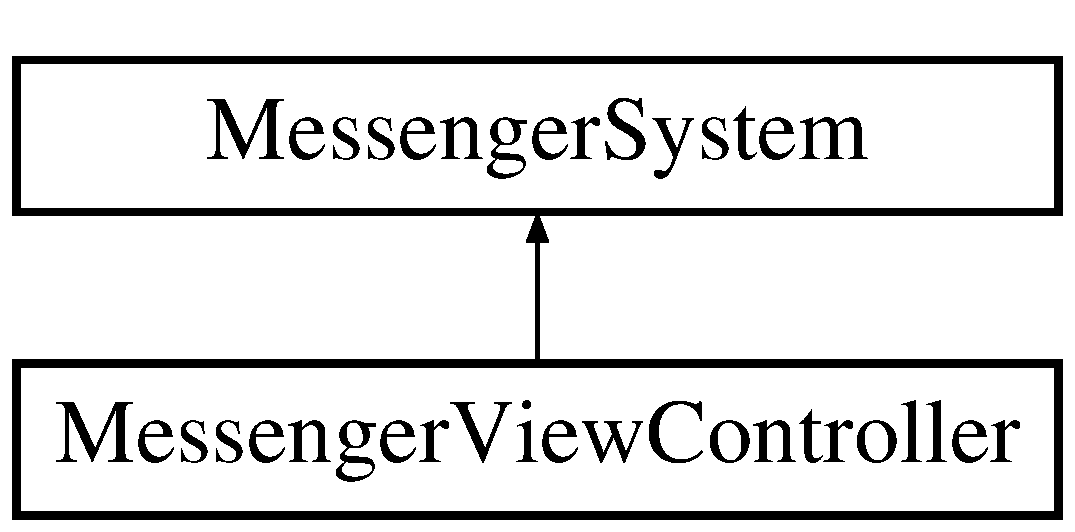
\includegraphics[height=2.000000cm]{d7/d34/interface_messenger_view_controller}
\end{center}
\end{figure}
\subsection*{Public メソッド}
\begin{DoxyCompactItemize}
\item 
(id) -\/ \hyperlink{interface_messenger_view_controller_a44c0a2552e50d6223a8230447be3e83a}{initWithBodyID:withSelector:withName:}
\item 
(id) -\/ \hyperlink{interface_messenger_view_controller_a1ac23270dbc04a95b72dd16b2c201c5a}{initWithFrame:}
\item 
(void) -\/ \hyperlink{interface_messenger_view_controller_aa30151ef1d95034a10fa31e9c8a7da22}{insertMessengerInformation:withMID:}
\item 
(void) -\/ \hyperlink{interface_messenger_view_controller_a3eb404c4ef5fc51caae10e71136f35ff}{updateParentInformation:withMID:withParentName:withParentMID:}
\item 
(void) -\/ \hyperlink{interface_messenger_view_controller_ab9c9343a0f520cdc1aa91b3985b31f7a}{deleteMessengerInformation:withMID:}
\item 
(void) -\/ \hyperlink{interface_messenger_view_controller_aba89f37600bb5cc7258a034614257dc6}{drawDataUpdate}
\item 
(NSString $\ast$) -\/ \hyperlink{interface_messenger_view_controller_a9c958b9ee93a81551b3aa4209eaa3c71}{getMessengerInformationKey:withMID:}
\item 
(NSMutableDictionary $\ast$) -\/ \hyperlink{interface_messenger_view_controller_afa883d1d29e91d003087a0f4b839daf3}{getButtonList}
\item 
(NSMutableDictionary $\ast$) -\/ \hyperlink{interface_messenger_view_controller_a2e4617fc57087279158f9df78fab0a87}{getMessengerList}
\item 
(void) -\/ \hyperlink{interface_messenger_view_controller_aa75f66a06d37f03a7d2b51e9c7149051}{setNumberOfRelationship:}
\item 
\hypertarget{interface_messenger_view_controller_aa06b18307f500c793a8493da0969b57b}{
(int) -\/ {\bfseries getNumberOfRelationship}}
\label{d7/d34/interface_messenger_view_controller_aa06b18307f500c793a8493da0969b57b}

\item 
(UIView $\ast$) -\/ \hyperlink{interface_messenger_view_controller_ae7d3fbe4156df4e7f1539f50500f0919}{getMessengerInterfaceView}
\item 
(void) -\/ \hyperlink{interface_messenger_view_controller_a008c7cc6364c75b6f70ef3d79fa3a043}{tapped:}
\item 
(void) -\/ \hyperlink{interface_messenger_view_controller_a61c88e671203c5651b89394f3b300285}{resizeButton:}
\item 
(void) -\/ \hyperlink{interface_messenger_view_controller_afe36a73932b47fb2c60412c6f03f67ac}{setMyName:}
\item 
(void) -\/ \hyperlink{interface_messenger_view_controller_abab9347cc7ed46bd04978ca00e081a0e}{setMyBodyID:}
\item 
(void) -\/ \hyperlink{interface_messenger_view_controller_ade8005d21b7d8df69ddd12fba7440f6b}{setMyBodySelector:}
\item 
(void) -\/ \hyperlink{interface_messenger_view_controller_a2c2f7a46b94facbc66d66c7dd6da34bd}{initMyMID}
\item 
(void) -\/ \hyperlink{interface_messenger_view_controller_a5728b61e9c4490af7aacddd874026bae}{initMyParentData}
\item 
(void) -\/ \hyperlink{interface_messenger_view_controller_a9d6939385be720d5335fbf5b095cd63c}{setMyParentName:}
\item 
(void) -\/ \hyperlink{interface_messenger_view_controller_a791916fe5a33b084e90d14cd12d9bc30}{setNameIndexDictionary}
\item 
\hypertarget{interface_messenger_view_controller_a27a84207c430e3402014720823e7b7dd}{
(NSMutableDictionary $\ast$) -\/ {\bfseries getNameIndexDictionary}}
\label{d7/d34/interface_messenger_view_controller_a27a84207c430e3402014720823e7b7dd}

\item 
(void) -\/ \hyperlink{interface_messenger_view_controller_a6c8d083521df8a95e9e88612745d5981}{sortButtonsByParentOrder}
\item 
(void) -\/ \hyperlink{interface_messenger_view_controller_a3939f43ce30df6b8df0390712730282b}{setWorldX:withY:}
\item 
\hypertarget{interface_messenger_view_controller_a48556e3f4bded903ba3080d2411ce5ec}{
(void) -\/ {\bfseries moveWorldX:withY:}}
\label{d7/d34/interface_messenger_view_controller_a48556e3f4bded903ba3080d2411ce5ec}

\item 
\hypertarget{interface_messenger_view_controller_a4f8fb574a6997e9f92731c32a4155c77}{
(void) -\/ {\bfseries setScale:}}
\label{d7/d34/interface_messenger_view_controller_a4f8fb574a6997e9f92731c32a4155c77}

\item 
\hypertarget{interface_messenger_view_controller_a97b35c6553c0ec2e6aae62ec4f4e8db4}{
(float) -\/ {\bfseries getScale}}
\label{d7/d34/interface_messenger_view_controller_a97b35c6553c0ec2e6aae62ec4f4e8db4}

\item 
(void) -\/ \hyperlink{interface_messenger_view_controller_a9a0f05d1d3a3685a3d3ce7632c2bc7ee}{scaleResetX:withY:}
\item 
(void) -\/ \hyperlink{interface_messenger_view_controller_a33bb3cca76fba84a3e5b480131e5faf1}{inputParent:}
\item 
(void) -\/ \hyperlink{interface_messenger_view_controller_a2c415df83e46605177105d75c714e463}{innerPerform:}
\item 
(void) -\/ \hyperlink{interface_messenger_view_controller_a416d9acd2e8346b9ab8870b64571f322}{callMyself:}
\item 
(void) -\/ \hyperlink{interface_messenger_view_controller_a7a416a5ec2bcd17f259e1b2fc017d6a6}{call:withExec:}
\item 
\hypertarget{interface_messenger_view_controller_a95e335be7444d6a9fd4631fa8a5f9f3e}{
(void) -\/ {\bfseries callChild:withMID:withCommand:}}
\label{d7/d34/interface_messenger_view_controller_a95e335be7444d6a9fd4631fa8a5f9f3e}

\item 
(void) -\/ \hyperlink{interface_messenger_view_controller_afa8cf33ccddb2f83e214b192707bdbd6}{callParent:}
\item 
\hypertarget{interface_messenger_view_controller_ae8415c3e0079cb51a8374a47efa0bbd2}{
(void) -\/ {\bfseries createdNotice}}
\label{d7/d34/interface_messenger_view_controller_ae8415c3e0079cb51a8374a47efa0bbd2}

\item 
\hypertarget{interface_messenger_view_controller_a975afc92bea2290fcae8b57ab85985d3}{
(void) -\/ {\bfseries updatedNotice:withParentMID:}}
\label{d7/d34/interface_messenger_view_controller_a975afc92bea2290fcae8b57ab85985d3}

\item 
\hypertarget{interface_messenger_view_controller_abf4d1e2b5e6cd851f60601482ec500ef}{
(void) -\/ {\bfseries killedNotice}}
\label{d7/d34/interface_messenger_view_controller_abf4d1e2b5e6cd851f60601482ec500ef}

\item 
(void) -\/ \hyperlink{interface_messenger_view_controller_a764894e696ddb4254c216dbb8d58b279}{dealloc}
\end{DoxyCompactItemize}
\subsection*{Protected 変数}
\begin{DoxyCompactItemize}
\item 
\hypertarget{interface_messenger_view_controller_aa7a06978c9d2e2580a0cd3b19467c204}{
NSMutableDictionary $\ast$ {\bfseries m\_\-messengerList}}
\label{d7/d34/interface_messenger_view_controller_aa7a06978c9d2e2580a0cd3b19467c204}

\item 
\hypertarget{interface_messenger_view_controller_afb79d57e4d89d863e81dc6bf77e33d7d}{
NSMutableDictionary $\ast$ {\bfseries m\_\-buttonList}}
\label{d7/d34/interface_messenger_view_controller_afb79d57e4d89d863e81dc6bf77e33d7d}

\item 
\hypertarget{interface_messenger_view_controller_a70f8ee629bb1e1c67dc0e74389d29c29}{
NSMutableDictionary $\ast$ {\bfseries m\_\-nameIndexDictionary}}
\label{d7/d34/interface_messenger_view_controller_a70f8ee629bb1e1c67dc0e74389d29c29}

\item 
\hypertarget{interface_messenger_view_controller_a8cbd0807ee7f3d3a50ad46cfb6dfed21}{
\hyperlink{interface_messenger_display_view}{MessengerDisplayView} $\ast$ {\bfseries messengerInterfaceView}}
\label{d7/d34/interface_messenger_view_controller_a8cbd0807ee7f3d3a50ad46cfb6dfed21}

\item 
\hypertarget{interface_messenger_view_controller_af273157267a9808e9bb252e3a43f80c6}{
int {\bfseries m\_\-numberOfRelationship}}
\label{d7/d34/interface_messenger_view_controller_af273157267a9808e9bb252e3a43f80c6}

\item 
\hypertarget{interface_messenger_view_controller_a5e7ee1ec43301204e1ef57fb7a3e0153}{
float {\bfseries m\_\-scale}}
\label{d7/d34/interface_messenger_view_controller_a5e7ee1ec43301204e1ef57fb7a3e0153}

\item 
\hypertarget{interface_messenger_view_controller_abf360a74ed5bfcfcc0e2e5d9ca883e4f}{
float {\bfseries m\_\-worldX}}
\label{d7/d34/interface_messenger_view_controller_abf360a74ed5bfcfcc0e2e5d9ca883e4f}

\item 
\hypertarget{interface_messenger_view_controller_a99f4c4324081b5a093411151cb82bb96}{
float {\bfseries m\_\-worldY}}
\label{d7/d34/interface_messenger_view_controller_a99f4c4324081b5a093411151cb82bb96}

\end{DoxyCompactItemize}


\subsection{関数}
\hypertarget{interface_messenger_view_controller_a7a416a5ec2bcd17f259e1b2fc017d6a6}{
\index{MessengerViewController@{MessengerViewController}!call:withExec:@{call:withExec:}}
\index{call:withExec:@{call:withExec:}!MessengerViewController@{MessengerViewController}}
\subsubsection[{call:withExec:}]{\setlength{\rightskip}{0pt plus 5cm}-\/ (void) call: 
\begin{DoxyParamCaption}
\item[{dummy(NSString $\ast$)}]{ childName}
\item[{withExec:(NSString $\ast$)}]{ exec}
\item[{,}]{ ...}
\end{DoxyParamCaption}
}}
\label{d7/d34/interface_messenger_view_controller_a7a416a5ec2bcd17f259e1b2fc017d6a6}
特定の名前のmessengerへの通信を行うメソッド 異なる名前の親から子へのメッセージ限定 

\hyperlink{interface_messenger_system_ae9f0c6c7daf251eb28aad584b1eca292}{MessengerSystem}を再定義しています。

\hypertarget{interface_messenger_view_controller_a416d9acd2e8346b9ab8870b64571f322}{
\index{MessengerViewController@{MessengerViewController}!callMyself:@{callMyself:}}
\index{callMyself:@{callMyself:}!MessengerViewController@{MessengerViewController}}
\subsubsection[{callMyself:}]{\setlength{\rightskip}{0pt plus 5cm}-\/ (void) callMyself: 
\begin{DoxyParamCaption}
\item[{dummy(NSString $\ast$)}]{ exec}
\item[{,}]{ ...}
\end{DoxyParamCaption}
}}
\label{d7/d34/interface_messenger_view_controller_a416d9acd2e8346b9ab8870b64571f322}
自分自身のmessengerへと通信を行うメソッド 

\hyperlink{interface_messenger_system_a0d78a7be460a84be04e67d73ddcf4248}{MessengerSystem}を再定義しています。

\hypertarget{interface_messenger_view_controller_afa8cf33ccddb2f83e214b192707bdbd6}{
\index{MessengerViewController@{MessengerViewController}!callParent:@{callParent:}}
\index{callParent:@{callParent:}!MessengerViewController@{MessengerViewController}}
\subsubsection[{callParent:}]{\setlength{\rightskip}{0pt plus 5cm}-\/ (void) callParent: 
\begin{DoxyParamCaption}
\item[{dummy(NSString $\ast$)}]{ exec}
\item[{,}]{ ...}
\end{DoxyParamCaption}
}}
\label{d7/d34/interface_messenger_view_controller_afa8cf33ccddb2f83e214b192707bdbd6}
親への通信を行うメソッド 

\hyperlink{interface_messenger_system_acf758deab41281c54d928be2a72fc9ba}{MessengerSystem}を再定義しています。

\hypertarget{interface_messenger_view_controller_a764894e696ddb4254c216dbb8d58b279}{
\index{MessengerViewController@{MessengerViewController}!dealloc@{dealloc}}
\index{dealloc@{dealloc}!MessengerViewController@{MessengerViewController}}
\subsubsection[{dealloc}]{\setlength{\rightskip}{0pt plus 5cm}-\/ (void) dealloc 
\begin{DoxyParamCaption}
{}
\end{DoxyParamCaption}
}}
\label{d7/d34/interface_messenger_view_controller_a764894e696ddb4254c216dbb8d58b279}
Dealloc \hypertarget{interface_messenger_view_controller_ab9c9343a0f520cdc1aa91b3985b31f7a}{
\index{MessengerViewController@{MessengerViewController}!deleteMessengerInformation:withMID:@{deleteMessengerInformation:withMID:}}
\index{deleteMessengerInformation:withMID:@{deleteMessengerInformation:withMID:}!MessengerViewController@{MessengerViewController}}
\subsubsection[{deleteMessengerInformation:withMID:}]{\setlength{\rightskip}{0pt plus 5cm}-\/ (void) deleteMessengerInformation: 
\begin{DoxyParamCaption}
\item[{dummy(NSString $\ast$)}]{ senderName}
\item[{withMID:(NSString $\ast$)}]{ senderMID}
\end{DoxyParamCaption}
}}
\label{d7/d34/interface_messenger_view_controller_ab9c9343a0f520cdc1aa91b3985b31f7a}
通信してきた対象の情報をviwDictから削除するメソッド

メッセンジャーの削除をビューに反映する \hypertarget{interface_messenger_view_controller_aba89f37600bb5cc7258a034614257dc6}{
\index{MessengerViewController@{MessengerViewController}!drawDataUpdate@{drawDataUpdate}}
\index{drawDataUpdate@{drawDataUpdate}!MessengerViewController@{MessengerViewController}}
\subsubsection[{drawDataUpdate}]{\setlength{\rightskip}{0pt plus 5cm}-\/ (void) drawDataUpdate 
\begin{DoxyParamCaption}
{}
\end{DoxyParamCaption}
}}
\label{d7/d34/interface_messenger_view_controller_aba89f37600bb5cc7258a034614257dc6}
描画データのアップデート

ドローデータの更新 \hypertarget{interface_messenger_view_controller_afa883d1d29e91d003087a0f4b839daf3}{
\index{MessengerViewController@{MessengerViewController}!getButtonList@{getButtonList}}
\index{getButtonList@{getButtonList}!MessengerViewController@{MessengerViewController}}
\subsubsection[{getButtonList}]{\setlength{\rightskip}{0pt plus 5cm}-\/ (NSMutableDictionary $\ast$) getButtonList 
\begin{DoxyParamCaption}
{}
\end{DoxyParamCaption}
}}
\label{d7/d34/interface_messenger_view_controller_afa883d1d29e91d003087a0f4b839daf3}
ボタン、Messengerのリスト辞書を渡す

ボタン用の辞書を取得する \hypertarget{interface_messenger_view_controller_a9c958b9ee93a81551b3aa4209eaa3c71}{
\index{MessengerViewController@{MessengerViewController}!getMessengerInformationKey:withMID:@{getMessengerInformationKey:withMID:}}
\index{getMessengerInformationKey:withMID:@{getMessengerInformationKey:withMID:}!MessengerViewController@{MessengerViewController}}
\subsubsection[{getMessengerInformationKey:withMID:}]{\setlength{\rightskip}{0pt plus 5cm}-\/ (NSString $\ast$) getMessengerInformationKey: 
\begin{DoxyParamCaption}
\item[{dummy(NSString $\ast$)}]{ name}
\item[{withMID:(NSString $\ast$)}]{ MID}
\end{DoxyParamCaption}
}}
\label{d7/d34/interface_messenger_view_controller_a9c958b9ee93a81551b3aa4209eaa3c71}
NameとMIDのペアを作るメソッド \hypertarget{interface_messenger_view_controller_ae7d3fbe4156df4e7f1539f50500f0919}{
\index{MessengerViewController@{MessengerViewController}!getMessengerInterfaceView@{getMessengerInterfaceView}}
\index{getMessengerInterfaceView@{getMessengerInterfaceView}!MessengerViewController@{MessengerViewController}}
\subsubsection[{getMessengerInterfaceView}]{\setlength{\rightskip}{0pt plus 5cm}-\/ (UIView $\ast$) getMessengerInterfaceView 
\begin{DoxyParamCaption}
{}
\end{DoxyParamCaption}
}}
\label{d7/d34/interface_messenger_view_controller_ae7d3fbe4156df4e7f1539f50500f0919}
ビューを返す

Viewを外部に返す \hypertarget{interface_messenger_view_controller_a2e4617fc57087279158f9df78fab0a87}{
\index{MessengerViewController@{MessengerViewController}!getMessengerList@{getMessengerList}}
\index{getMessengerList@{getMessengerList}!MessengerViewController@{MessengerViewController}}
\subsubsection[{getMessengerList}]{\setlength{\rightskip}{0pt plus 5cm}-\/ (NSMutableDictionary $\ast$) getMessengerList 
\begin{DoxyParamCaption}
{}
\end{DoxyParamCaption}
}}
\label{d7/d34/interface_messenger_view_controller_a2e4617fc57087279158f9df78fab0a87}
View用の辞書を取得する \hypertarget{interface_messenger_view_controller_a2c2f7a46b94facbc66d66c7dd6da34bd}{
\index{MessengerViewController@{MessengerViewController}!initMyMID@{initMyMID}}
\index{initMyMID@{initMyMID}!MessengerViewController@{MessengerViewController}}
\subsubsection[{initMyMID}]{\setlength{\rightskip}{0pt plus 5cm}-\/ (void) initMyMID 
\begin{DoxyParamCaption}
{}
\end{DoxyParamCaption}
}}
\label{d7/d34/interface_messenger_view_controller_a2c2f7a46b94facbc66d66c7dd6da34bd}
自分のMIDを初期化するメソッド \hypertarget{interface_messenger_view_controller_a5728b61e9c4490af7aacddd874026bae}{
\index{MessengerViewController@{MessengerViewController}!initMyParentData@{initMyParentData}}
\index{initMyParentData@{initMyParentData}!MessengerViewController@{MessengerViewController}}
\subsubsection[{initMyParentData}]{\setlength{\rightskip}{0pt plus 5cm}-\/ (void) initMyParentData 
\begin{DoxyParamCaption}
{}
\end{DoxyParamCaption}
}}
\label{d7/d34/interface_messenger_view_controller_a5728b61e9c4490af7aacddd874026bae}
myParent関連情報を初期化する \hypertarget{interface_messenger_view_controller_a44c0a2552e50d6223a8230447be3e83a}{
\index{MessengerViewController@{MessengerViewController}!initWithBodyID:withSelector:withName:@{initWithBodyID:withSelector:withName:}}
\index{initWithBodyID:withSelector:withName:@{initWithBodyID:withSelector:withName:}!MessengerViewController@{MessengerViewController}}
\subsubsection[{initWithBodyID:withSelector:withName:}]{\setlength{\rightskip}{0pt plus 5cm}-\/ (id) initWithBodyID: 
\begin{DoxyParamCaption}
\item[{dummy(id)}]{ body\_\-id}
\item[{withSelector:(SEL)}]{ body\_\-selector}
\item[{withName:(NSString $\ast$)}]{ name}
\end{DoxyParamCaption}
}}
\label{d7/d34/interface_messenger_view_controller_a44c0a2552e50d6223a8230447be3e83a}
使用禁止の初期化メソッド 

\hyperlink{interface_messenger_system_a1127377a8d677d41693b435758790e79}{MessengerSystem}を再定義しています。

\hypertarget{interface_messenger_view_controller_a1ac23270dbc04a95b72dd16b2c201c5a}{
\index{MessengerViewController@{MessengerViewController}!initWithFrame:@{initWithFrame:}}
\index{initWithFrame:@{initWithFrame:}!MessengerViewController@{MessengerViewController}}
\subsubsection[{initWithFrame:}]{\setlength{\rightskip}{0pt plus 5cm}-\/ (id) initWithFrame: 
\begin{DoxyParamCaption}
\item[{dummy(CGRect)}]{ frame}
\end{DoxyParamCaption}
}}
\label{d7/d34/interface_messenger_view_controller_a1ac23270dbc04a95b72dd16b2c201c5a}
初期化メソッド \hypertarget{interface_messenger_view_controller_a2c415df83e46605177105d75c714e463}{
\index{MessengerViewController@{MessengerViewController}!innerPerform:@{innerPerform:}}
\index{innerPerform:@{innerPerform:}!MessengerViewController@{MessengerViewController}}
\subsubsection[{innerPerform:}]{\setlength{\rightskip}{0pt plus 5cm}-\/ (void) innerPerform: 
\begin{DoxyParamCaption}
\item[{dummy(NSNotification $\ast$)}]{ notification}
\end{DoxyParamCaption}
}}
\label{d7/d34/interface_messenger_view_controller_a2c415df83e46605177105d75c714e463}
内部処理実装 オーバーライドし、実行内容を限定する \hypertarget{interface_messenger_view_controller_a33bb3cca76fba84a3e5b480131e5faf1}{
\index{MessengerViewController@{MessengerViewController}!inputParent:@{inputParent:}}
\index{inputParent:@{inputParent:}!MessengerViewController@{MessengerViewController}}
\subsubsection[{inputParent:}]{\setlength{\rightskip}{0pt plus 5cm}-\/ (void) inputParent: 
\begin{DoxyParamCaption}
\item[{dummy(NSString $\ast$)}]{ parentName}
\end{DoxyParamCaption}
}}
\label{d7/d34/interface_messenger_view_controller_a33bb3cca76fba84a3e5b480131e5faf1}
親へと自分が子供である事の通知を行い、返り値として親のMIDをmyParentMIDとして受け取るメソッド 受け取り用のメソッドの情報を親へと渡し、親からの遠隔MID入力を受ける。 

\hyperlink{interface_messenger_system_a2dc1b363d2e1b00f232fd829225a9ff3}{MessengerSystem}を再定義しています。

\hypertarget{interface_messenger_view_controller_aa30151ef1d95034a10fa31e9c8a7da22}{
\index{MessengerViewController@{MessengerViewController}!insertMessengerInformation:withMID:@{insertMessengerInformation:withMID:}}
\index{insertMessengerInformation:withMID:@{insertMessengerInformation:withMID:}!MessengerViewController@{MessengerViewController}}
\subsubsection[{insertMessengerInformation:withMID:}]{\setlength{\rightskip}{0pt plus 5cm}-\/ (void) insertMessengerInformation: 
\begin{DoxyParamCaption}
\item[{dummy(NSString $\ast$)}]{ senderName}
\item[{withMID:(NSString $\ast$)}]{ senderMID}
\end{DoxyParamCaption}
}}
\label{d7/d34/interface_messenger_view_controller_aa30151ef1d95034a10fa31e9c8a7da22}
メッセンジャーの生成情報をviewDictへと保持しておくメソッド

メッセンジャーの誕生をビューに反映する \hypertarget{interface_messenger_view_controller_a61c88e671203c5651b89394f3b300285}{
\index{MessengerViewController@{MessengerViewController}!resizeButton:@{resizeButton:}}
\index{resizeButton:@{resizeButton:}!MessengerViewController@{MessengerViewController}}
\subsubsection[{resizeButton:}]{\setlength{\rightskip}{0pt plus 5cm}-\/ (void) resizeButton: 
\begin{DoxyParamCaption}
\item[{dummy(UIButton $\ast$)}]{ b}
\end{DoxyParamCaption}
}}
\label{d7/d34/interface_messenger_view_controller_a61c88e671203c5651b89394f3b300285}
ボタンのインフォメーションを書き換え、再度描画 

ここからのラインを確認する。 通信の宛先に繋がっているラインをピックアップ、 別途アップデートにかける。どうでもいいか。

第一優先を色、完了 第二優先を→、線の上につける、かなあ、 第三優先を拡大縮小にしようか。画面のピッチに対する倍率を持てばいい。

グローバル基点と、グローバルスケールを持つ。アップデートをタッチ離したときに取ればいい。

\hypertarget{interface_messenger_view_controller_a9a0f05d1d3a3685a3d3ce7632c2bc7ee}{
\index{MessengerViewController@{MessengerViewController}!scaleResetX:withY:@{scaleResetX:withY:}}
\index{scaleResetX:withY:@{scaleResetX:withY:}!MessengerViewController@{MessengerViewController}}
\subsubsection[{scaleResetX:withY:}]{\setlength{\rightskip}{0pt plus 5cm}-\/ (void) scaleResetX: 
\begin{DoxyParamCaption}
\item[{dummy(float)}]{ x}
\item[{withY:(float)}]{ y}
\end{DoxyParamCaption}
}}
\label{d7/d34/interface_messenger_view_controller_a9a0f05d1d3a3685a3d3ce7632c2bc7ee}
ビューからの直結イベント ズームインかリセットを行う \hypertarget{interface_messenger_view_controller_abab9347cc7ed46bd04978ca00e081a0e}{
\index{MessengerViewController@{MessengerViewController}!setMyBodyID:@{setMyBodyID:}}
\index{setMyBodyID:@{setMyBodyID:}!MessengerViewController@{MessengerViewController}}
\subsubsection[{setMyBodyID:}]{\setlength{\rightskip}{0pt plus 5cm}-\/ (void) setMyBodyID: 
\begin{DoxyParamCaption}
\item[{dummy(id)}]{ bodyID}
\end{DoxyParamCaption}
}}
\label{d7/d34/interface_messenger_view_controller_abab9347cc7ed46bd04978ca00e081a0e}
自分のBodyIDをセットするメソッド 

\hyperlink{interface_messenger_system_a2a5f63ed86009e8b451bbbb621e9a94b}{MessengerSystem}を再定義しています。

\hypertarget{interface_messenger_view_controller_ade8005d21b7d8df69ddd12fba7440f6b}{
\index{MessengerViewController@{MessengerViewController}!setMyBodySelector:@{setMyBodySelector:}}
\index{setMyBodySelector:@{setMyBodySelector:}!MessengerViewController@{MessengerViewController}}
\subsubsection[{setMyBodySelector:}]{\setlength{\rightskip}{0pt plus 5cm}-\/ (void) setMyBodySelector: 
\begin{DoxyParamCaption}
\item[{dummy(SEL)}]{ body\_\-selector}
\end{DoxyParamCaption}
}}
\label{d7/d34/interface_messenger_view_controller_ade8005d21b7d8df69ddd12fba7440f6b}
自分のBodyが提供するメソッドセレクターを、自分のセレクター用ポインタにセットするメソッド 

\hyperlink{interface_messenger_system_aafb5a2e5d48a09627f32a4d3c2e3fa29}{MessengerSystem}を再定義しています。

\hypertarget{interface_messenger_view_controller_afe36a73932b47fb2c60412c6f03f67ac}{
\index{MessengerViewController@{MessengerViewController}!setMyName:@{setMyName:}}
\index{setMyName:@{setMyName:}!MessengerViewController@{MessengerViewController}}
\subsubsection[{setMyName:}]{\setlength{\rightskip}{0pt plus 5cm}-\/ (void) setMyName: 
\begin{DoxyParamCaption}
\item[{dummy(NSString $\ast$)}]{ name}
\end{DoxyParamCaption}
}}
\label{d7/d34/interface_messenger_view_controller_afe36a73932b47fb2c60412c6f03f67ac}
自分の名称をセットするメソッド \hypertarget{interface_messenger_view_controller_a9d6939385be720d5335fbf5b095cd63c}{
\index{MessengerViewController@{MessengerViewController}!setMyParentName:@{setMyParentName:}}
\index{setMyParentName:@{setMyParentName:}!MessengerViewController@{MessengerViewController}}
\subsubsection[{setMyParentName:}]{\setlength{\rightskip}{0pt plus 5cm}-\/ (void) setMyParentName: 
\begin{DoxyParamCaption}
\item[{dummy(NSString $\ast$)}]{ parent}
\end{DoxyParamCaption}
}}
\label{d7/d34/interface_messenger_view_controller_a9d6939385be720d5335fbf5b095cd63c}
親の名称をセットするメソッド \hypertarget{interface_messenger_view_controller_a791916fe5a33b084e90d14cd12d9bc30}{
\index{MessengerViewController@{MessengerViewController}!setNameIndexDictionary@{setNameIndexDictionary}}
\index{setNameIndexDictionary@{setNameIndexDictionary}!MessengerViewController@{MessengerViewController}}
\subsubsection[{setNameIndexDictionary}]{\setlength{\rightskip}{0pt plus 5cm}-\/ (void) setNameIndexDictionary 
\begin{DoxyParamCaption}
{}
\end{DoxyParamCaption}
}}
\label{d7/d34/interface_messenger_view_controller_a791916fe5a33b084e90d14cd12d9bc30}
表示補助用のインデックス X軸カウント \hypertarget{interface_messenger_view_controller_aa75f66a06d37f03a7d2b51e9c7149051}{
\index{MessengerViewController@{MessengerViewController}!setNumberOfRelationship:@{setNumberOfRelationship:}}
\index{setNumberOfRelationship:@{setNumberOfRelationship:}!MessengerViewController@{MessengerViewController}}
\subsubsection[{setNumberOfRelationship:}]{\setlength{\rightskip}{0pt plus 5cm}-\/ (void) setNumberOfRelationship: 
\begin{DoxyParamCaption}
\item[{dummy(int)}]{ number}
\end{DoxyParamCaption}
}}
\label{d7/d34/interface_messenger_view_controller_aa75f66a06d37f03a7d2b51e9c7149051}
関係性の本数を返すメソッド \hypertarget{interface_messenger_view_controller_a3939f43ce30df6b8df0390712730282b}{
\index{MessengerViewController@{MessengerViewController}!setWorldX:withY:@{setWorldX:withY:}}
\index{setWorldX:withY:@{setWorldX:withY:}!MessengerViewController@{MessengerViewController}}
\subsubsection[{setWorldX:withY:}]{\setlength{\rightskip}{0pt plus 5cm}-\/ (void) setWorldX: 
\begin{DoxyParamCaption}
\item[{dummy(float)}]{ toX}
\item[{withY:(float)}]{ toY}
\end{DoxyParamCaption}
}}
\label{d7/d34/interface_messenger_view_controller_a3939f43ce30df6b8df0390712730282b}
移動、スケール関連

平行移動、スケールに関する処理 \hypertarget{interface_messenger_view_controller_a6c8d083521df8a95e9e88612745d5981}{
\index{MessengerViewController@{MessengerViewController}!sortButtonsByParentOrder@{sortButtonsByParentOrder}}
\index{sortButtonsByParentOrder@{sortButtonsByParentOrder}!MessengerViewController@{MessengerViewController}}
\subsubsection[{sortButtonsByParentOrder}]{\setlength{\rightskip}{0pt plus 5cm}-\/ (void) sortButtonsByParentOrder 
\begin{DoxyParamCaption}
{}
\end{DoxyParamCaption}
}}
\label{d7/d34/interface_messenger_view_controller_a6c8d083521df8a95e9e88612745d5981}
全ボタンの位置をソートする

一番左からソートをかける 親子関係のラインから、キーに入っているオブジェクトに重み付け、m\_\-nameIndexDictionary 内のX軸カウントを先頭に持っていく \hypertarget{interface_messenger_view_controller_a008c7cc6364c75b6f70ef3d79fa3a043}{
\index{MessengerViewController@{MessengerViewController}!tapped:@{tapped:}}
\index{tapped:@{tapped:}!MessengerViewController@{MessengerViewController}}
\subsubsection[{tapped:}]{\setlength{\rightskip}{0pt plus 5cm}-\/ (void) tapped: 
\begin{DoxyParamCaption}
\item[{dummy(UIControlEvents $\ast$)}]{ event}
\end{DoxyParamCaption}
}}
\label{d7/d34/interface_messenger_view_controller_a008c7cc6364c75b6f70ef3d79fa3a043}
ボタンが押された際のメソッド

ボタンが押された時のメソッド \hypertarget{interface_messenger_view_controller_a3eb404c4ef5fc51caae10e71136f35ff}{
\index{MessengerViewController@{MessengerViewController}!updateParentInformation:withMID:withParentName:withParentMID:@{updateParentInformation:withMID:withParentName:withParentMID:}}
\index{updateParentInformation:withMID:withParentName:withParentMID:@{updateParentInformation:withMID:withParentName:withParentMID:}!MessengerViewController@{MessengerViewController}}
\subsubsection[{updateParentInformation:withMID:withParentName:withParentMID:}]{\setlength{\rightskip}{0pt plus 5cm}-\/ (void) updateParentInformation: 
\begin{DoxyParamCaption}
\item[{dummy(NSString $\ast$)}]{ senderName}
\item[{withMID:(NSString $\ast$)}]{ senderMID}
\item[{withParentName:(NSString $\ast$)}]{ sendersParentName}
\item[{withParentMID:(NSString $\ast$)}]{ sendersParentMID}
\end{DoxyParamCaption}
}}
\label{d7/d34/interface_messenger_view_controller_a3eb404c4ef5fc51caae10e71136f35ff}
通信してきた対象の情報をviewDictへと保持しておくメソッド

通信してきた対象の情報がアップデートされ、親情報が変更された

正確に更新が行われていれば、線が残るような事は発生しない筈。 

このクラスの説明は次のファイルから生成されました:\begin{DoxyCompactItemize}
\item 
Classes/MessengerSystem/MessengerViewController.h\item 
Classes/MessengerSystem/MessengerViewController.m\end{DoxyCompactItemize}

\printindex
\end{document}
